\chapter{Background}\label{ch:background}

\section{Digital Twins}

A \acrfull{dt} is a physical and/or virtual machines or computer-based model that simulate, emulate, mirror, or ``twin'' the life of a physical entity, which may be an object, a process, a human, or a human-related feature \parencite{barricelliMultiModalApproachCreating2022}.

Far from a passive copy, a \acrshort{dt} is an intelligent and adaptive entity, acting as the living counterpart to its physical twin~\parencite{grievesDigitalTwinManufacturing2015,kritzingerDigitalTwinManufacturing2018}. It continuously monitors, analyzes, and optimizes the real-world process or object throughout its lifecycle. This not only allows for proactive maintenance and prevention of issues like defects and failures, but also enables experimentation and optimization through simulations of new configurations. The twinning process is allowed by the dynamic interplay between the digital twin, its physical counterpart, and the surrounding environment --- a continuous loop of interaction, communication, and refinement.

The \acrshort{dt} maintains continual awareness of its physical counterpart and surrounding environment through real-time data streams and extensive data storage capabilities. Descriptive data exchanges, facilitated by big data infrastructure, ensure consistent synchronization with the physical system. Advanced algorithms, including data fusion, big data analytics, and \acrshort{ai}-based descriptive methods, are applied to extract valuable insights from this rich data pool. The modular and highly parameterized architecture of the \acrshort{dt} enables rapid reconfiguration, allowing it to evolve alongside its physical twin. This synchronization ensures the \acrshort{dt} constantly reflects the properties and changes occurring in the real world.

Leveraging its \acrshort{ai} capabilities, the \acrshort{dt} transcends mere emulation by uncovering hidden patterns, unknown correlations, and comprehensive system descriptions. This holistic understanding of the physical system, combined with the ability to record, control, and monitor its condition, enables techniques for failure forecasting, simulation of potential solutions, and even activation of self-healing mechanisms. This powerful combination facilitates a predictive maintenance approach, where proactive interventions prevent failures and optimize performance through simulated testing and solution selection.

Despite their inherent intelligence, \acrshort{dt}s are not designed to operate in complete autonomy. \acrshort{ai}-based applications and \acrshort{dt}s often require significant human intervention, particularly when testing novel features and modifications on physical assets, as well as when the systems are leveraged to provide crucial outputs like medical diagnoses and treatment recommendations~\parencite{barricelliSurveyDigitalTwin2019}.

\subsection{Historical Notes}

The concept of \acrshort{dt} first appeared in the field of \acrfull{plm}, where it was informally introduced in 2002 by Michael Grieves, and later formalized \parencite{grievesDigitalTwinManufacturing2015,grievesDigitalTwinMitigating2017}. Grieves’ \acrshort{dt} model, represented in Figure~\ref{fig:grieves_digital_twin} was composed by three primary elements:
\begin{enumerate}
    \item A real space containing a physical object;
    \item A virtual space containing a virtual object;
    \item The link for data flow from real space to virtual space (and virtual sub-spaces), and for information flow from virtual space (and sub-spaces) to real space. This last element is the enabler of data exchange, thus allowing the convergence and synchronization of the virtual and physical systems.
\end{enumerate}

\begin{figure}
    \centering
    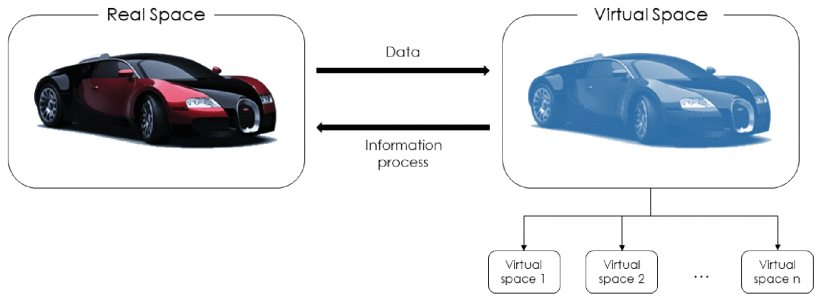
\includegraphics[width=0.8\textwidth]{images/dt_model_grieves.png}
    \caption{Grieves' digital twin model}{Grieves' digital twin model. From \cite{barricelliSurveyDigitalTwin2019}, \textit{Research Background} section, CC-BY 4.0 license.}
    \label{fig:grieves_digital_twin}
\end{figure}

A later development was proposed by \cite{framlingProductAgentsHandling2003}, who proposed ``an agent-based architecture where each product item has a corresponding virtual counterpart or agent associated with it''. Exploiting the seamless connection provided by the spread of Internet technologies, the envisioned agents should guarantee the synchronization with their physical counterpart, providing also services for them~\parencite{framlingProductAgentsHandling2003}. The authors' proposal is based on the consideration that an effective \acrshort{plm} system should always have access to a faithful view of the product status and information, from when it is planned and manufactured, through its time of use, and until the time of disposal.

Following Grieves' definition, \acrshort{dt}s garnered much interest in the aerospace and defense industries.
NASA researched \acrshort{dt}s as a way to reduce costs and resources for its space assets. Their investigation lead to a roadmap that confirmed the vale of \acrshort{dt}s in improving performance in the field of aviation. The authors defined the DT as ``an integrated multi-physics, multi-scale, probabilistic simulation of a vehicle or system that uses the best available physical models, sensor updates, fleet history, etc., to mirror the life of its flying twin. The digital twin is ultra-realistic and may consider one or more important and interdependent vehicle systems, including propulsion/energy storage, avionics, life support, vehicle structure, thermal management/TPS, etc.''~\parencite{shaftoModelingSimulationInformation2010}. The U.S. Air Force also developed the \acrfull{adt}, a computational model of individual aircrafts, which had the potential to improve the way U.S. Air Force aircrafts were managed over their entire lifecycle by creating individualized structural management plans~\parencite{tuegelAirframeDigitalTwin2012,gockelChallengesStructuralLife2012}.

\acrshort{dt}s also are key point of Industry 4.0~\parencite{brettelHowVirtualizationDecentralization2014,hermannDesignPrinciplesIndustrie2016,vachalekDigitalTwinIndustrial2017} and Smart Manufacturing~\parencite{mabkhotRequirementsSmartFactory2018}.

\subsection{Characteristics of Digital Twins}

Seamless and reliable communication is fundamental to \acrshort{dt} functionality. Both physical and virtual twins require networking devices to facilitate continuous data exchange, achieved either through direct physical connections or indirect cloud-based networks. This facilitates a constant flow of information from the physical twin, which describes the physical twin status and change with time along its lifecycle, along with dynamic environment data describing the surrounding environment status. Furthermore, the \acrshort{dt} actively transmits predictions for maintenance, optimizations, insights, and recommendations for improved function to the physical twin, human specialists, and to other \acrshort{dt}s in its environment. As such, three key communication processes must be designed:

\begin{enumerate}
    \item Physical-\acrshort{dt}. This direct exchange ensures real-time synchronization between the physical system and its digital representation.
    \item \acrshort{dt}-to-\acrshort{dt}: This enables collaboration and knowledge sharing between multiple digital twins within the interconnected environment.
    \item \acrshort{dt}-Expert: User-friendly interfaces facilitate interaction and operation of the \acrshort{dt} by domain experts, maximizing the value derived from this data-driven technology.
\end{enumerate}

The \acrshort{dt} relies on a robust data storage system to house the continuously streamed sensor data reflecting the real-time status and changes of the physical twin.
It also memorizes historical static data, which reflect the physical twin memory and record historical information provided by human expertise or by past actions, and descriptive static data, that captures essential, unchanging characteristics of the physical twin. To comprehend and formalize this diverse data, the \acrshort{dt} leverages proper ontologies, ensuring consistent interpretation and efficient utilization.

Given the complexity of captured data, the \acrshort{dt} employs techniques for high-dimensional data (de-)coding and analysis, which are tailored to process and analyze complex, multi-dimensional data structures. It also requires data fusion algorithms, to integrate data from various sources like sensors and historical records, providing a holistic understanding of the physical system.

The \acrshort{dt} includes various \acrshort{ai} algorithms, whose predictive capabilities are constantly refined. Supervised and/or unsupervised machine learning models to classify and categorize data points based on past observations and known patterns. Their predictive capability is refined as they process the continuously received sensed data from the physical twin and the surrounding environment. Feature selection and extraction methods are used to reduce the data dimensionality while keeping the most informative data, enahncing computational efficiency.

Finally, the \acrshort{dt} has self-adaptation and self-parametrization capabilities, to adjust its internal parameters to keep pace with the evolving physical twin throughout its lifecycle. It also exploits predictive analytics to predict future statuses, important changes, and to recommend optimal actions and interventions. When making future predictions, it must take into account uncertainties in the data. At any time, it should offer a real-time view of the physical system's condition, and enable simulation and exploration of potential \textit{what-if} scenarios under various conditions, supporting informed decision-making.

\subsection{Design of a Digital Twin}

This study led us to describe two possible lifecycles for DTs, from their design to their dismissal. The former refers to a case where the object that has to be twinned still does not exist and, in this case, the design process simultaneously conceives both the object and its DT. The latter is about an object that already exists but has no DT in place; in this case, the design process focuses on the extension of the objects to make it connected.

Both lifecycles share the same timeline: a first Design phase, followed by a Development phase, an Operational phase, and finally a Dismissal phase. For describing these two lifecycles, we use a running example of a medical device (the object) – i.e. a computer tomography scanner. The first lifecycle is shown in Fig. 3. In this first case, the DT starts living before the physical object as a Prototype (Prototype DTObject), which is then used by designers during the Design phase of the Prototype Object. During the initial part of the Design phase, the Prototype DTObject is used, as if it was the real prototype, to simulate, test, change, and eventually validate design choices, until the best solution is found. During this part of the design phase, designers exploit: 1) Historical data the Prototype DTObject acquires from any other already existing DTs linked to similar devices. 2) Static data (e.g., data describing the product requirements, customer preferences, bill of materials). 3) The results of simulations performed by the Prototype DTObject, the result of predictions computed by the Prototype DTObject, and its suggestions and optimization schema. When the design of Prototype DTObject is completed, the process moves to the Design of the prototype Object, during which the Prototype DTObject is eventually modified to address technical constraints that may arise during the prototyping of the physical Object. During the Development Phase, the Prototype DTObject evolves becoming a Development DTObject, which must interact with the production machines to follow and optimize the assembly/construction of the Object, i.e. its physical twin. When the Object is finally built, the Development DTObject starts being a Product DTObject, and this moves the process into the Operational phase. The Product DTObject fully resembles the Object: it has the AI acquired by the preceding stages of its life, and is therefore ready to follow and mirror the medical device (Object) while it is being used. During its existence, the intelligence of the DTObject grows and self-adapts to the Object (in the case of the medical equipment, for example, it might start learning the most requested examinations, and the days when more or less examinations are performed). When the Object stops being used (due to obsolescence or any other reason) it must be disassembled, and the Dismissal phase begins, first for the Object and then for the DTObject. The stored historical data of the Product DTObject are backed-up and made available to other DTObject as well as to domain experts; in this way, designers, or any other domain expert, will be able to use the collected information to optimize the production of future devices. The second lifecycle is shown in Fig. 4. The difference between this lifecycle and the previous one (Fig. 3), is that the Object is already in place and in use, but it does not have a connected DT yet. In this case, the Design phase regards the development of a novel Prototype DTObject (which is tested, changed and finally validated), the Development phase regards the development of connections between the existing Object and the DTObject (which is called Development DTObject in this phase), while the Operational phase regards the operational life of the two twins, the Connected Object and Product DTObject, which live in concert until their dismantle in the Dismissal phase. To sum up, during their lifecycle, the (physical and digital) twins base each step of their existence on a synergic and continuous interaction, which allow monitoring, predicting, and optimizing all their functionalities. The continuous interaction hides the differences among them, and they can act as a whole (‘‘Synergy is the creation of a whole that is greater than the sum of its parts’’ [129]).

\begin{itemize}
    \item Opportunities and challenges of digital twins
    \item Digital twins for sustainability
\end{itemize}

\section{Virtual Assistants}

\subsection{Routines}

\begin{itemize}
    \item Definition of virtual assistant
    \item IoT ecosystems
\end{itemize}